

\setcounter{section}{2}
\section{System Components}
\bigskip

\subsection{MCU - ESP32}
\medskip
ESP32 is a series of low-cost, low-power system on a chip microcontrollers with integrated Wi-Fi and dual-mode Bluetooth. Created and developed by Espressif, the ESP32 contains a Tensilica Xtensa LX6 microprocessor in both dual-core and single-core variations and includes a in-built antenna, power amplifier, low-noise receive amplifier, filters, and power-management modules (As shown in figure \ref{esp_core}) \cite{R3-1-1}. 

\medskip
\begin{figure}[H]
\centering
    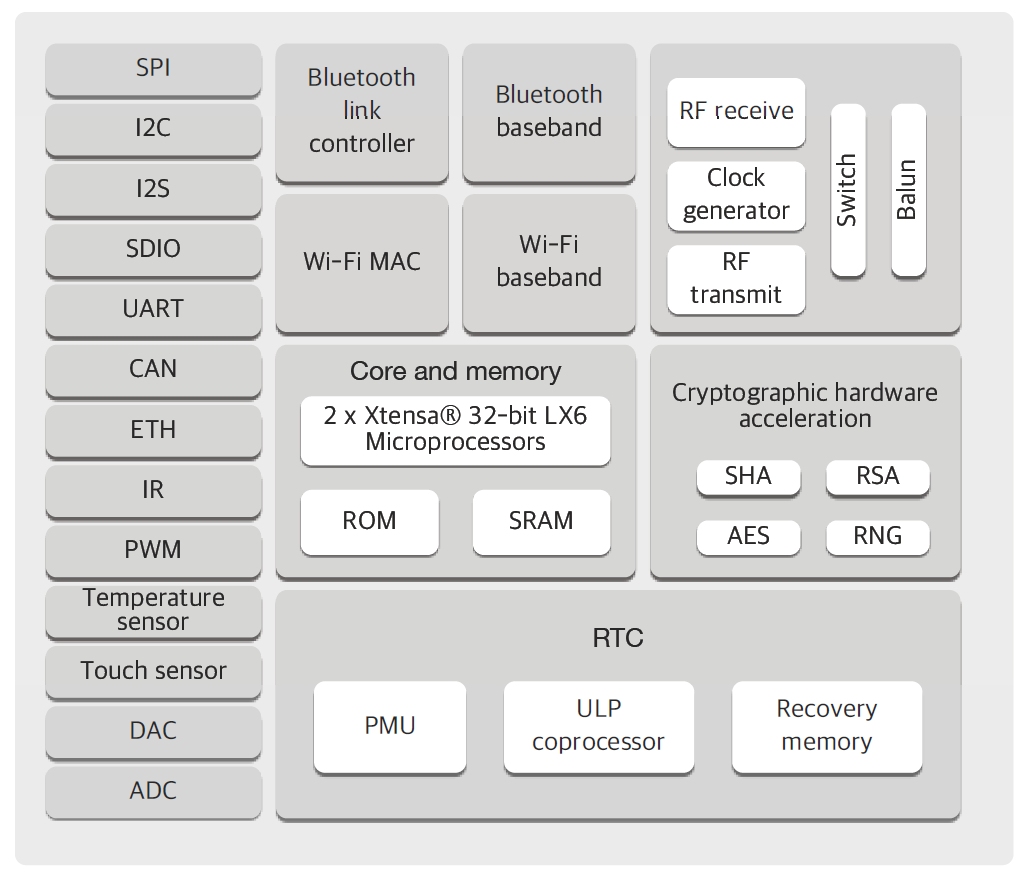
\includegraphics[scale=0.4]{./images/esp_core.png}
    \caption{ESP32 Architect Block Diagram}
    \label{esp_core}
\end{figure}

For the proof of concept, the Bluetooth modules on the ESP32 will be used as the communication interface between the Beacon and the ID tags. Using BLE advertising, the ID Tags ESP32 broadcasts a unique MAC address. The Beacon ESP32 can collect all assicating ID Tag ESP32s and capture the RSSI and MAC of these devices. These information are forwarded to the DPU for distances establition and location plotting.

\begin{figure}[H]
\centering
    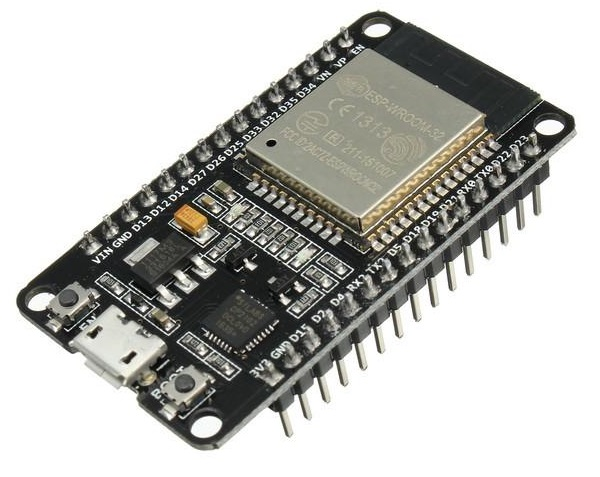
\includegraphics[scale=0.25]{./images/esp.jpg}
    \caption{ESP32 Development Board}
    \label{esp}
\end{figure}


\pagebreak
In the Final design the ESP32 will be incorporated as the main controller unit for both the beacons and ID tags but with Decawave DWM1000 UWB modules as the transceiver. For the beacons the ESP32’s Serial Peripheral Interface (SPI) will be used to interact with the Decawave DWM1000 UWB modules. As for the ID Tags, the ESP32 features a deep sleep mode which reduces power consumption to about 10uA from 260mA (active operations), thus drastically increasing the battery life time. Furthermore, with its wide range of capabilities such as Wi-FI and Bluetooth, a mesh network and be implemented to extend the communication range of the Beacons. A mock-up circuit diagram presenting the SPI interface between the ESP32 and a breakout board for DWM1000 is shown in figure \ref{eps_dwm_circuit}.

\medskip
\begin{figure}[H]
\centering
    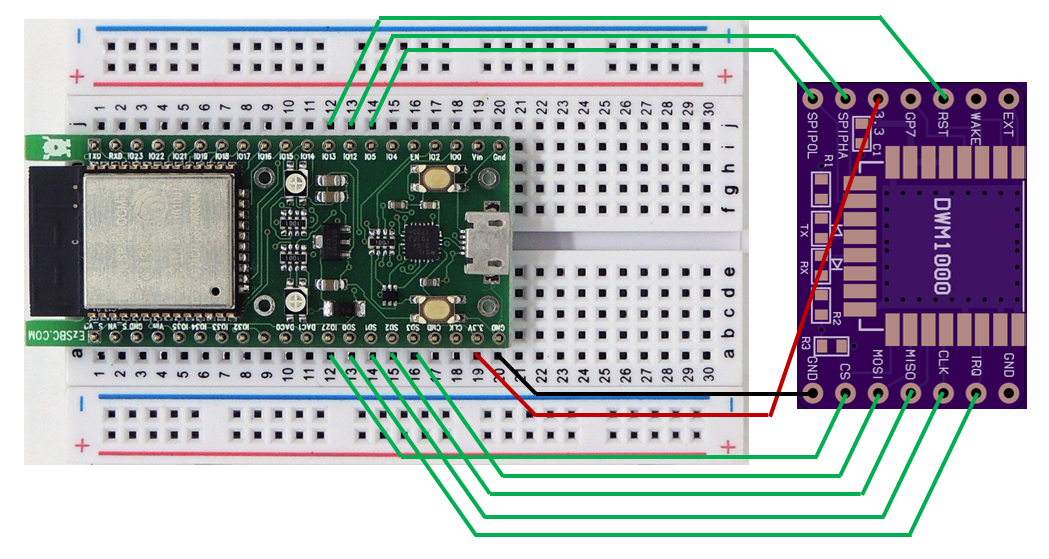
\includegraphics[scale=0.5]{./images/eps_dwm_circuit.png}
    \caption{Circuit Diagram of ESP32 \& DWM1000}
    \label{eps_dwm_circuit}
\end{figure}



\pagebreak
\subsection{Transceiver - DWM1000} 
\medskip
The Beacon and ID Tag communication will be done using ultra-wideband wireless communication. The most optimal transceiver available on the market that most fits the needs and scope of this project is the Decawave DWM1000 UWB module (Figure \ref{dwm1000}). The DWM1000 is an IEEE802.15.4-2011 UWB compliant and FCC/ETSI certified wireless transceiver module based on Decawave’s DW1000 IC \cite{R4-2-1}. This module is a combination of DW1000 IC, a built in antenna, power management system, and clock control for simple design integrations (Figure \ref{dwm1000_bd}). 

\medskip
\begin{figure}[H]
\centering
    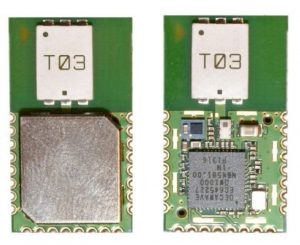
\includegraphics[scale=0.75]{./images/dwm1000.jpg}
    \caption{Decawave DWM1000 Modules}
    \label{dwm1000}
\end{figure}

The module enables the location tracking of objects in real time location systems (RTLS) to a precision of 10 cm indoors. It supports high range of communications data rates from 110 Kbps up to 6.8 Mbps, with excellent communication ranges of up to 300m. The frequencies of operation in the range of 3.5 GHz to 6.5 GHz with seven distinct channels which would significantly reduce issues of signal interference or multipath propagation. Its small physical size allows the module to be implemented in highly cost-effective solutions. By using this modul,e integration with the Akriveia Beacon system is intuitive and simple; since the DWM1000 also offers a wide range of MCU support such as Arduino MCUs or the ESP32 MCUs. 

\medskip
\begin{figure}[H]
\centering
    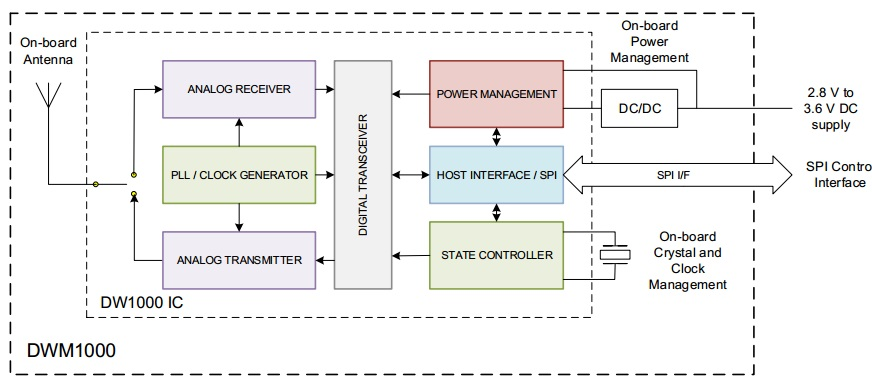
\includegraphics[scale=0.7]{./images/dwm1000_bd.jpg}
    \caption{DWM1000 Internal Block Diagram}
    \label{dwm1000_bd}
\end{figure}




\pagebreak
\subsection{DPU - Raspberry Pi}


\medskip
\begin{figure}[H]
\centering
    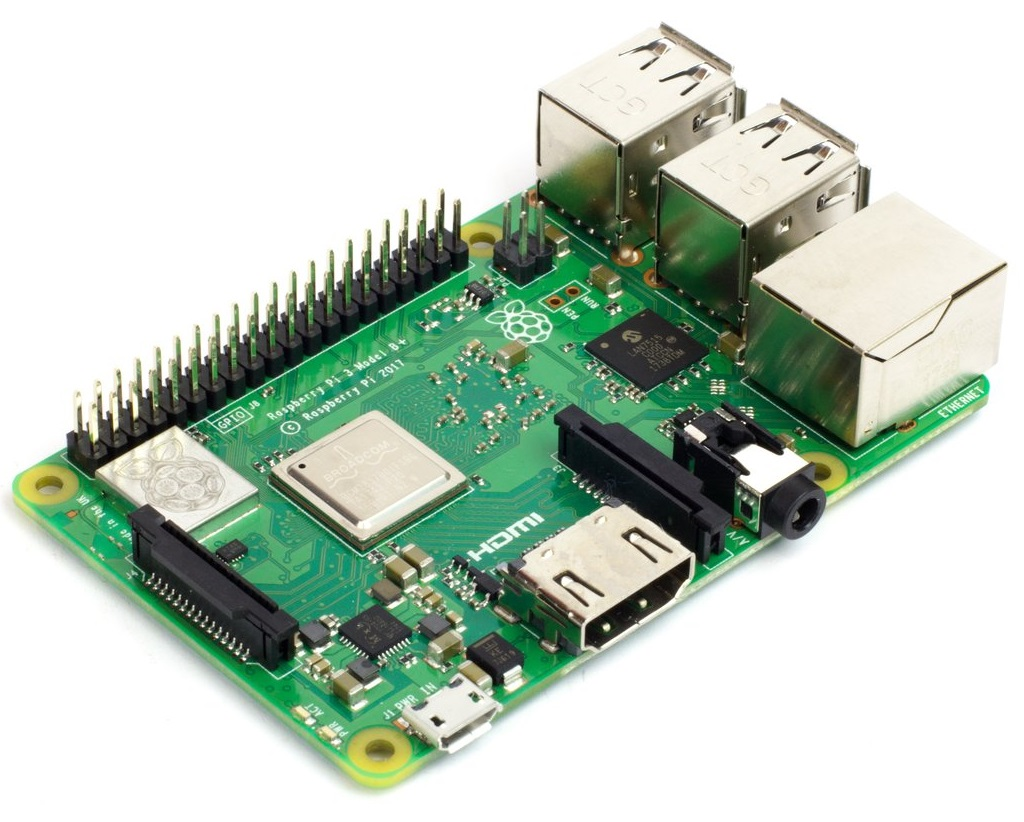
\includegraphics[scale=1]{./images/pi.jpg}
    \caption{Raspberry Pi 3 B+ Model}
    \label{pi}
\end{figure}




